\section{Results}

The main finding is consequence heterogeneity: a high pooled AUROC coexists with zero observed frameshift specificity. We first establish the paired protocol and its variability, then examine the stratum denominators and errors that qualify the pooled result.

\subsection{Small pooled effect of gene-component blocking}
Gene-component-blocked OOF evaluation yields 0.939 accuracy, 0.879 MCC, 0.984 AUROC, and 0.981 AP (Table~\ref{tab:primary}). Every sampled variant has a held-out prediction and no component crosses a blocked split. Test folds contain 3,712--4,210 rows, with pathogenic fractions 0.470--0.523. Accuracy ranges from 0.929 to 0.945; AUROC ranges from 0.979 to 0.987. In the random control, 2,549 components span multiple test folds and therefore also connect training and test data.

\begin{table*}[t]
\caption{OOF evaluations on the same 20,000 rows and separate holdout sensitivity. Original OOF arms use nested tuning; fixed-B random equals the original random arm. AF ranking supplies no threshold/probability metrics. Each holdout tests 4,000 variants. Entries are rounded independently; differences use unrounded values. Full precision is in the companion.}
\label{tab:primary}
\centering\footnotesize
\setlength{\tabcolsep}{3pt}
\begin{tabular}{@{}lrrrrrr@{}}
\toprule
Evaluation & Accuracy & MCC & AUROC & AP & Brier & ECE \\
\midrule
Random stratified, five-fold OOF & 0.943 & 0.885 & 0.985 & 0.982 & 0.043 & 0.009 \\
Gene-component-blocked, five-fold OOF & 0.939 & 0.879 & 0.984 & 0.981 & 0.046 & 0.014 \\
First-gene blocked, nested tuning & 0.940 & 0.879 & 0.984 & 0.981 & 0.046 & 0.016 \\
Component blocked, fixed B & 0.940 & 0.880 & 0.984 & 0.981 & 0.046 & 0.011 \\
Consequence-only logistic, blocked & 0.883 & 0.781 & 0.892 & 0.916 & 0.097 & 0.002 \\
AF-only ranking, blocked & -- & -- & 0.557 & 0.515 & -- & -- \\
\midrule
Random 80/20, ten-seed mean $\pm$ SD & $0.941\pm0.004$ & $0.882\pm0.009$ & $0.984\pm0.002$ & $0.981\pm0.003$ & $0.044\pm0.003$ & $0.015\pm0.004$ \\
\bottomrule
\end{tabular}
\end{table*}


Random-minus-blocked accuracy is 0.330 percentage points (pp; 95\% component-bootstrap interval 0.107--0.550 pp): 66 additional correct classifications among 20,000 rows. Discordant counts are 219 random-only correct and 153 blocked-only correct. AUROC decreases by 0.084 pp (0.027--0.141); the AP difference is 0.086 pp ($-0.019$--0.198), with an interval crossing zero (Fig.~\ref{fig:uncertainty}). Brier score increases from 0.043 to 0.046 and ECE from 0.009 to 0.014. Differences use unrounded values, not subtraction of rounded table entries.

\begin{figure*}[t]
\centering
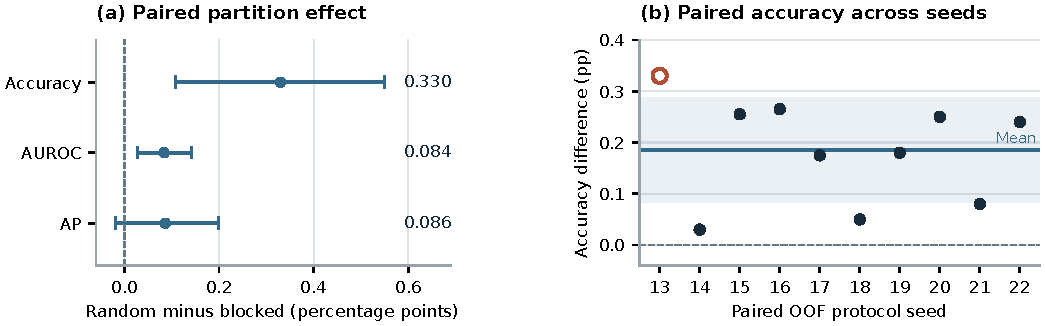
\includegraphics[width=\textwidth]{figures/split_and_seed_uncertainty.pdf}
\caption{(a) Seed-13 random-minus-blocked differences on identical OOF rows; bars: 95\% paired component-bootstrap intervals without refitting. Positive favors random splitting. (b) Accuracy differences from ten paired nested OOF runs, each refitting both arms on the same 20k sample; line: mean; shading: $\pm$ one sample SD, not a confidence interval; outline: seed 13. Units: percentage points (pp).}
\label{fig:uncertainty}
\end{figure*}

\subsection{Reproducibility across paired runs}
Across ten paired nested OOF runs, random-minus-blocked accuracy averages $0.186\pm0.102$ pp and AUROC $0.066\pm0.049$ pp (mean $\pm$ sample SD). Accuracy favors random splitting in 10/10 runs; AUROC in 9/10 (exploratory sign-test $p=0.002$ and $0.021$). The AP difference is $0.058\pm0.090$ pp, positive in 8/10 ($p=0.109$). The pooled partition effect is small and metric-dependent, with AUROC reversing in one run.

Separately, historical random-holdout accuracy is $0.94097\pm0.00441$; seed 13's 0.94675 is the maximum (range 0.93525--0.94675). The seed-13 OOF accuracy difference of 0.330 pp is smaller than this separate holdout SD of 0.441 pp. Comparing these distinct variability sources is descriptive, not a significance test; Fig.~\ref{fig:uncertainty}(b) directly repeats the paired contrast.

\subsection{Evidence dependence and comparator coverage}
Removing conservation/functional annotations reduces AUROC by 1.509 pp and MCC by 0.065. Removing population-frequency fields reduces them by 1.124 pp and 0.051. Amino-acid/BLOSUM62, consequence, and geometry/type removals produce AUROC drops of 0.247, 0.218, and 0.098 pp (Fig.~\ref{fig:evidence}). These quantify conditional predictive dependence under fixed full-model tuning.

Consequence-only logistic AUROC is 0.892 and AF-only ranking 0.557; 59.19\% of AF values are missing, limiting the latter baseline. First-gene-minus-component AUROC is $-0.006$ pp (95\% component interval $-0.060$--0.044), with no resolved incremental ranking benefit. Fixing B gives random-minus-component accuracy of 0.295 pp and AUROC of 0.085 pp (0.036--0.136), close to the nested contrast. Thus different selected configurations do not chiefly explain the seed-13 pooled effect.

\begin{table*}[t]
\caption{Exact-row comparisons, not a common leaderboard. Each score and the blocked local model (MX) use identical available rows. Coverage is relative to the 20,000-variant sample; $\pi$ is the subset's pathogenic fraction. Subsets differ between comparators, but not between models within a row.}
\label{tab:comparators}
\centering\footnotesize
\setlength{\tabcolsep}{6.2pt}
\begin{tabular}{@{}lrrrrrrr@{}}
\toprule
Score & Shared $n$ & Coverage (\%) & $\pi$ & MX AUROC & Score AUROC & MX AP & Score AP \\
\midrule
CADD & 15,015 & 75.1 & 0.368 & 0.983 & 0.967 & 0.970 & 0.946 \\
REVEL & 11,337 & 56.7 & 0.182 & 0.960 & 0.964 & 0.831 & 0.895 \\
AlphaMissense & 10,864 & 54.3 & 0.182 & 0.958 & 0.960 & 0.820 & 0.866 \\
\bottomrule
\end{tabular}
\end{table*}


On CADD's available rows, model-minus-comparator AUROC is 0.015 (95\% component interval 0.013--0.018), and AP is 0.025 (0.019--0.031). On REVEL's rows, the differences are $-0.004$ ($-0.010$--0.001) and $-0.064$ ($-0.089$--$-0.040$); on AlphaMissense's rows, $-0.002$ ($-0.007$--0.005) and $-0.046$ ($-0.072$--$-0.023$). REVEL and AlphaMissense have higher AP although their AUROC difference intervals cross zero. Both models share each comparison's prevalence, so different evaluation class fractions do not explain this AP gap. AP depends on ranking; strictly increasing recalibration preserves it. No retained comparator scores cover the 4,719 length-changing variants: an annotation-coverage gap, not evidence that CADD cannot score indels.

\subsection{What pooled performance conceals}
Global balance leaves unequal within-type class fractions (Table~\ref{tab:consequence}). Frameshift AP of 0.985 is close to its pathogenic fraction of 0.982, while AUROC is 0.563 (95\% component interval 0.491--0.633). All 68 benign frameshifts are called pathogenic; the nominal independent-row Wilson specificity interval is 0.000--0.053. In-frame deletion/insertion AUROCs are 0.490 (0.400--0.585) and 0.497 (0.342--0.643). Intervals including 0.5 indicate unresolved ranking evidence, not proof of equivalence to chance.

\begin{figure*}[t]
\centering
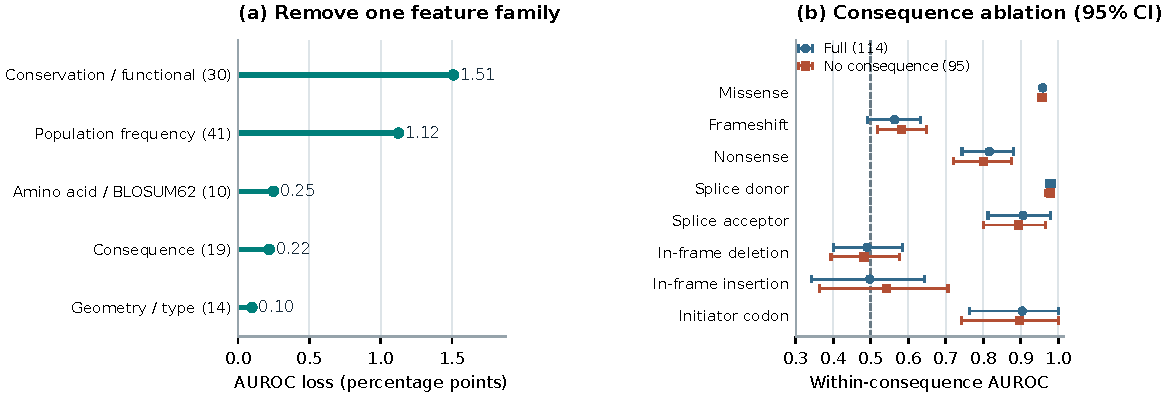
\includegraphics[width=\textwidth]{figures/evidence_and_consequences.pdf}
\caption{(a) AUROC loss after removing each feature family with fixed folds/configurations. (b) Full 114-field and consequence-drop 95-field models on identical rows: within-consequence AUROC with marginal 95\% component-bootstrap intervals (2,000 replicates, fixed predictions). The dashed line marks chance ranking. Intervals omit refitting uncertainty; paired differences are in the companion. Table~\ref{tab:consequence} supplies denominators and full-model threshold errors.}
\label{fig:evidence}
\end{figure*}

\begin{table*}[t]
\caption{Consequence-specific OOF results ($n\geq80$). P/B: pathogenic/benign including likely labels; $\pi=P/n$. Brackets: marginal 95\% component-bootstrap AUROC intervals (2,000 replicates within each stratum; fixed predictions, no refitting). Sensitivity/specificity use threshold 0.5. AP must be interpreted alongside $\pi$, particularly for frameshift and nonsense.}
\label{tab:consequence}
\centering\footnotesize
\setlength{\tabcolsep}{3.0pt}
\begin{tabular}{@{}lrrrrrrr@{}}
\toprule
Consequence & $n$ & P/B & $\pi$ & AP & AUROC [95\% CI] & Sens. & Spec. \\
\midrule
Missense & 11,614 & 2,026/9,588 & 0.174 & 0.815 & 0.958 [0.952, 0.964] & 0.742 & 0.955 \\
Frameshift & 3,856 & 3,788/68 & 0.982 & 0.985 & 0.563 [0.491, 0.633] & 1.000 & 0.000 \\
Nonsense & 2,505 & 2,450/55 & 0.978 & 0.992 & 0.816 [0.743, 0.880] & 0.996 & 0.364 \\
Splice donor & 878 & 836/42 & 0.952 & 0.999 & 0.980 [0.969, 0.989] & 0.993 & 0.619 \\
Splice acceptor & 750 & 713/37 & 0.951 & 0.987 & 0.906 [0.813, 0.979] & 0.996 & 0.486 \\
In-frame deletion & 185 & 68/117 & 0.368 & 0.402 & 0.490 [0.400, 0.585] & 0.132 & 0.932 \\
In-frame insertion & 87 & 21/66 & 0.241 & 0.295 & 0.497 [0.342, 0.643] & 0.095 & 0.970 \\
Initiator codon & 81 & 72/9 & 0.889 & 0.985 & 0.904 [0.764, 1.000] & 0.986 & 0.778 \\
\bottomrule
\end{tabular}
\end{table*}


Equation~\ref{eq:mixture} quantifies this composition effect. Of 100 million positive--negative pairs, 80.11\% cross consequence types. Their AUROC is 0.992; the within-consequence pair-weighted value is 0.952, combining to pooled 0.984. Missense supplies 97.67\% of within-consequence pairs, so this summary cannot represent rare strata uniformly. The identity describes where ranking comes from, not how much is caused by consequence features.

Removing the 19 consequence fields leaves frameshift specificity at zero. In-frame deletion sensitivity rises from 0.132 to 0.382, but specificity falls from 0.932 to 0.581 and AUROC remains near chance (0.481). This is a threshold trade-off, not recovered ranking; paired stratum ablation intervals are supplied in the companion.

\subsection{Probability and class-mix sensitivity}
The unstratified sample yields 0.981 AUROC, 0.988 AP, 0.045 Brier, and 0.022 ECE. Frameshift contains 5,124 pathogenic and 61 benign variants: specificity remains zero and AUROC is 0.452 (0.382--0.526). Missense AUROC is 0.960 (0.953--0.965); nonsense specificity is 0.316. The complete stratum results are in the companion. Thus the observed frameshift failure is not confined to the globally balanced sample, although sample composition, tuning, and weighting prevent a causal attribution to balancing.
